\section{Comparison across series of CV models}
\label{sxn:cv}


In this section, we examine quality metrics described in Section~\ref{sxn:methods} for several CV model architecture series.
This includes the VGG, ResNet, and DenseNet series of models, each of which consists of several pretrained DNN models, trained on the full ImageNet~\cite{imagenet} dataset, and each of which is distributed with the current opensource pyTorch framework (version 1.4)~\cite{pyTorch}.
This also includes a larger set of ResNet models, trained on the ImageNet-1K dataset~\cite{imagenet1k}, provided on the OSMR ``Sandbox for training convolutional networks for computer vision''~\cite{osmr}, which we call the ResNet-1K series.

We perform \emph{coarse model analysis}, comparing and contrasting the four model series, and predicting trends in model quality. 
We also perform \emph{fine layer analysis}, as a function of depth for these models, illustrating that PL-based metrics can provide novel insights among the VGG, ResNet/ResNet-1K, and DenseNet architectures. 

\paragraph{Coarse Analysis: Quality Metrics versus Reported Test Accuracies.}

We have examined the performance of the four quality metrics (Log Frobenius norm, Log Spectral norm, Weighted Alpha, and Log $\alpha$-Norm) applied to each of the VGG, ResNet, ResNet-1K, and DenseNet series.
To start, Figure~\ref{fig:vgg-metrics} considers the VGG series (in particular, the pretrained models VGG11, VGG13, VGG16, and VGG19, with and without BatchNormalization), and it plots the four quality metrics versus the reported Test accuracies~\cite{pyTorchVgg}, as well as a basic linear regression line. 
%with the Root Mean Squared Error (RMSE) shown, \michael{XXX.  WHERE IS RMSE.  IN THAT TABLE?}
All four metrics correlate quite well with the reported Top1 Accuracies, with smaller norms and smaller values of $\hat{\alpha}$ implying better generalziation (i.e., greater accuracy, lower error). 
While all four metrics perform well, notice that the Log $\alpha$-Norm metric ($\log\Vert\mathbf{W}\Vert_{\alpha}^{\alpha}$) performs best (with an RMSE of $0.42$, see Table~\ref{table:cv-models}); and the Weighted Alpha metric ($\hat\alpha =\alpha\log\lambda_{max} $), which is an approximation to the Log $\alpha$-Norm metric~\cite{MM20_unpub_work}, performs second best (with an RMSE of $0.48$, see Table~\ref{table:cv-models}).

\begin{figure}[t]
    \centering
    \subfigure[ Frobenius Norm, VGG ]{
        %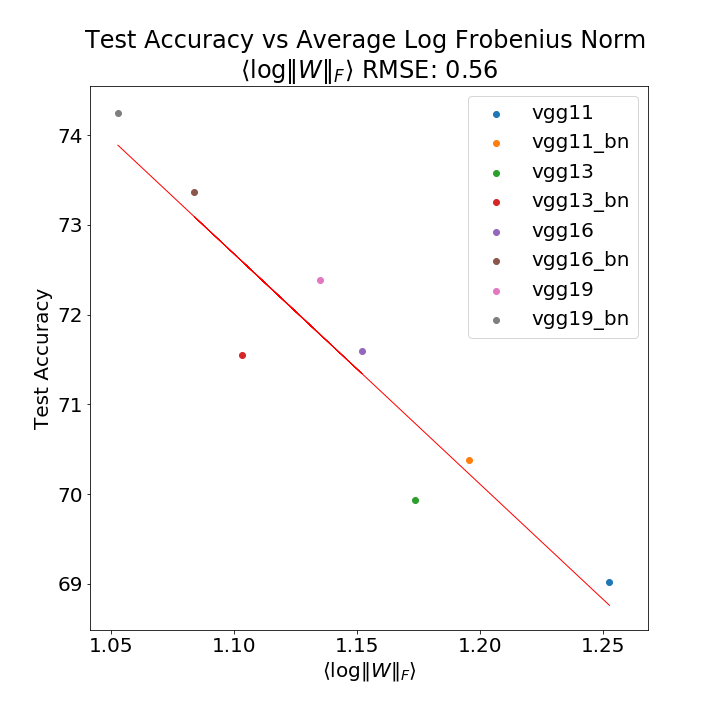
\includegraphics[width=5cm]{img/VGG_lognorm_accs.png}
        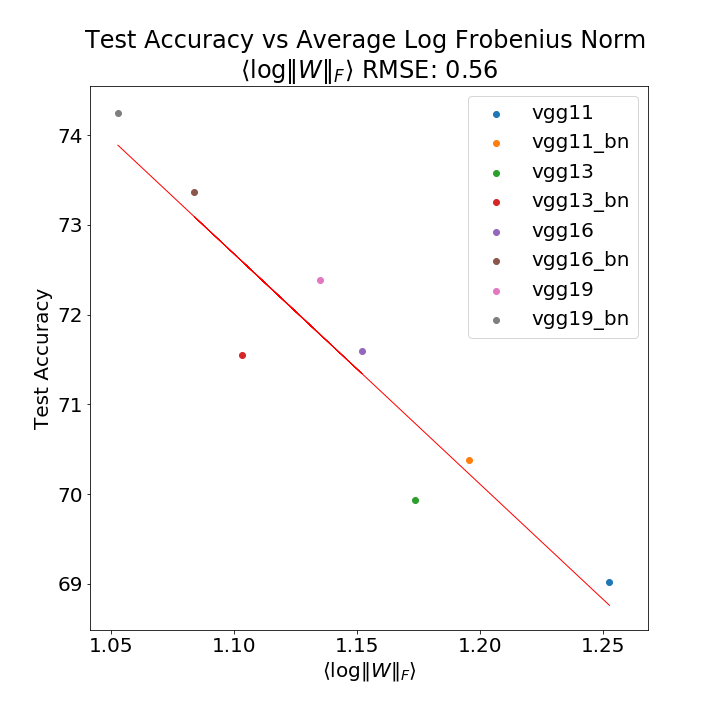
\includegraphics[width=3.7cm]{img/VGG_lognorm_accs.png}
        \label{fig:vgg-fnorm}
    }
    %\qquad
    \subfigure[ Spectral Norm, VGG ]{
        %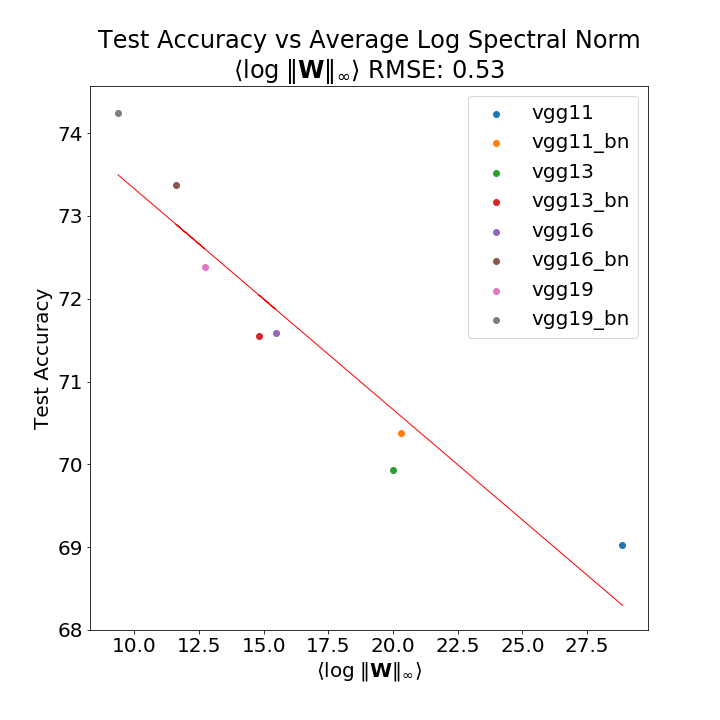
\includegraphics[width=4.9cm]{img/VGG_spectralnorm_accs.png}
        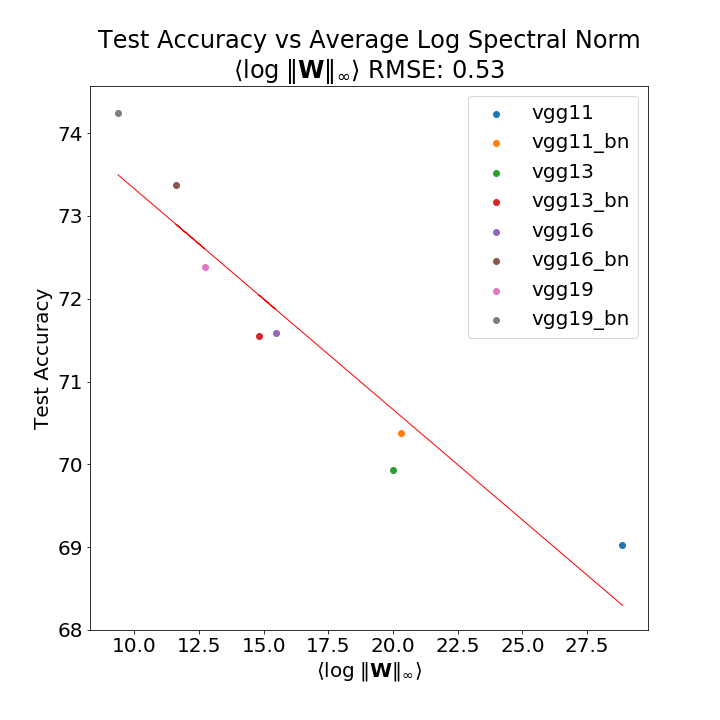
\includegraphics[width=3.7cm]{img/VGG_spectralnorm_accs.png}
        \label{fig:vgg-snorm}
    }
    %\qquad
    \subfigure[ Weighted Alpha, VGG ]{
        %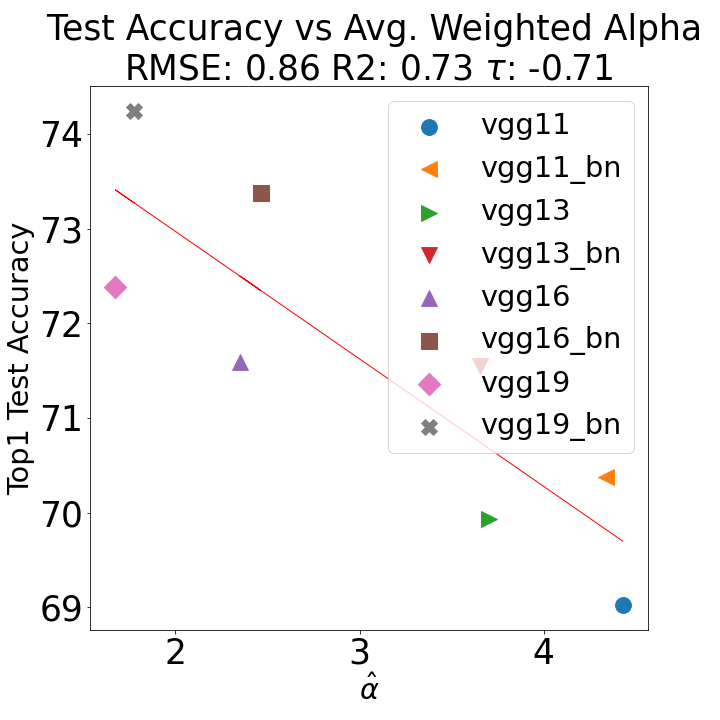
\includegraphics[width=4.9cm]{img/VGG_alpha_weighted_accs.png}
        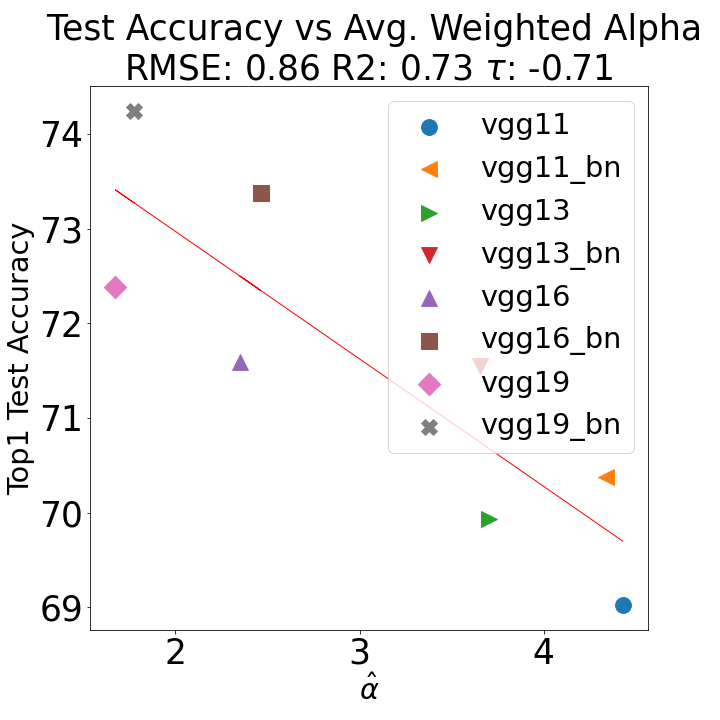
\includegraphics[width=3.7cm]{img/VGG_alpha_weighted_accs.png}
        \label{fig:vgg-walpha}
    }
    %\qquad
    \subfigure[ $\alpha$-Norm, VGG ]{
        %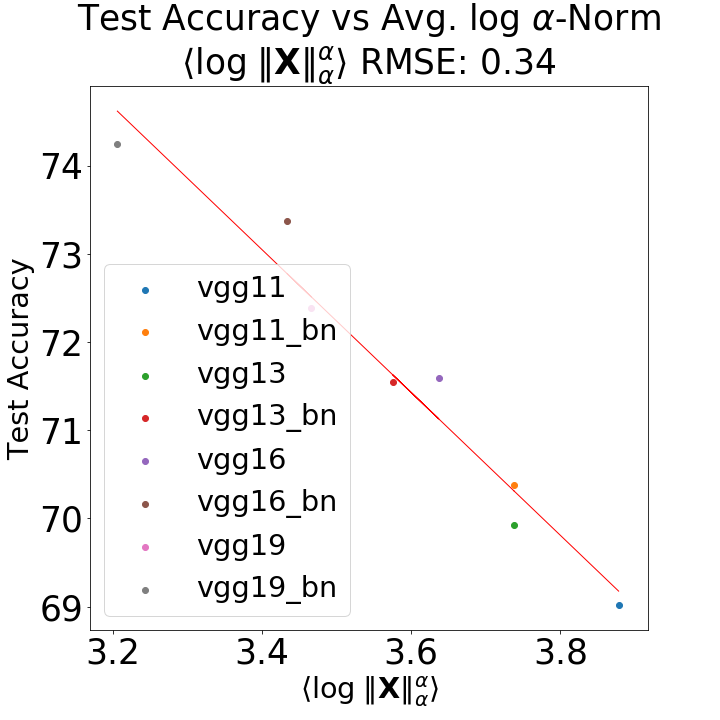
\includegraphics[width=4.9cm]{img/VGG_logpnorm_accs.png}
        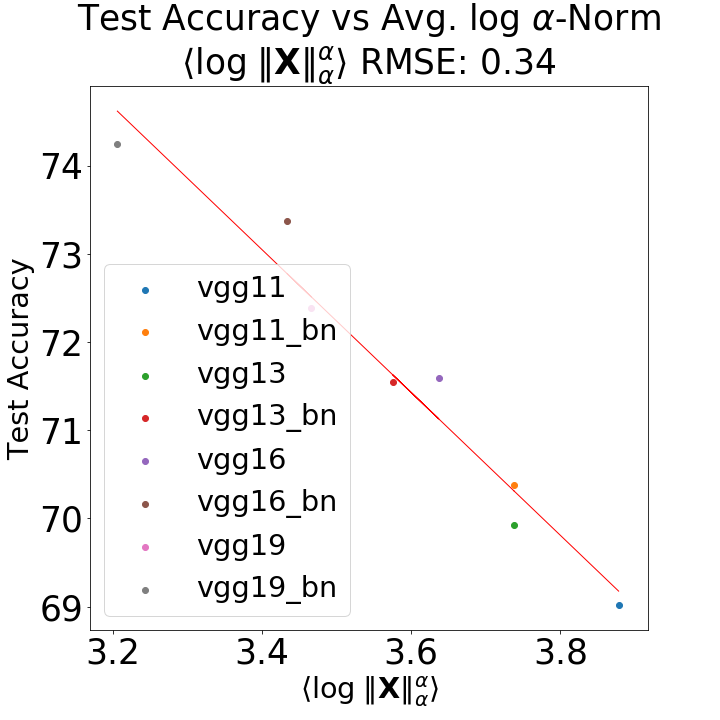
\includegraphics[width=3.7cm]{img/VGG_logpnorm_accs.png}
        \label{fig:vgg-pnorm}
    }
    \caption{Comparison of quality metrics versus reported test accuracy for pretrained VGG models, trained on ImageNet, available in pyTorch.  
             XXX Plots will be updated and replaced. 
             \michael{Figures are unreadable, can we make fonts bigger, etc.}
            }
    \label{fig:vgg-metrics}
\end{figure}


\begin{figure}[t]
    \centering

    \subfigure[ ResNet, $\alpha$-Norm ]{
        %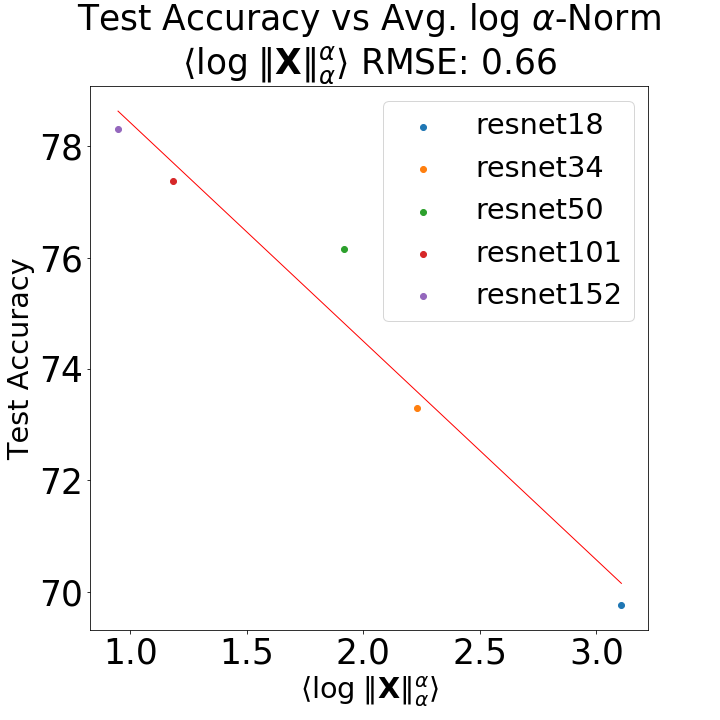
\includegraphics[width=4.2cm]{img/ResNet_logpnorm_accs.png}
        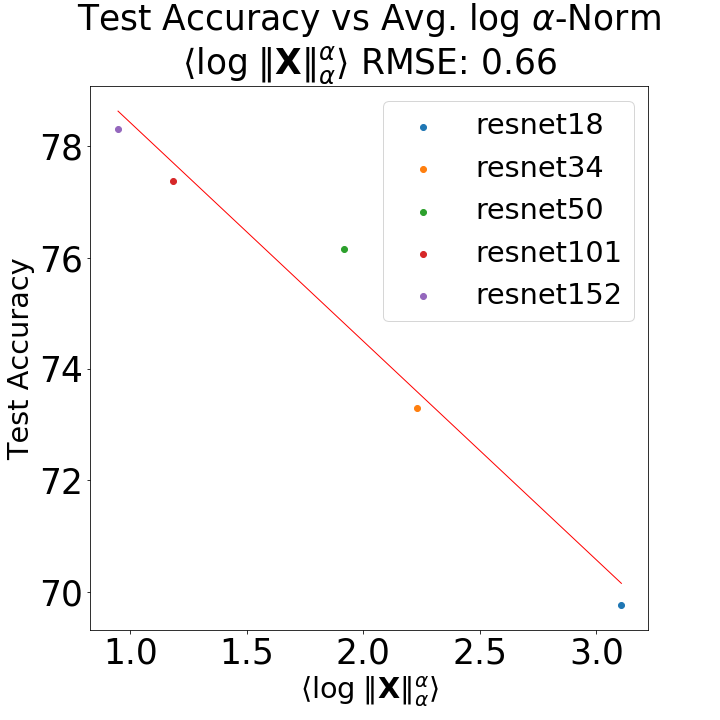
\includegraphics[width=3.7cm]{img/ResNet_logpnorm_accs.png}
        \label{fig:resnet-accuracy}
    }
    \qquad
    \subfigure[ ResNet-1K, $\alpha$-Norm ]{
        %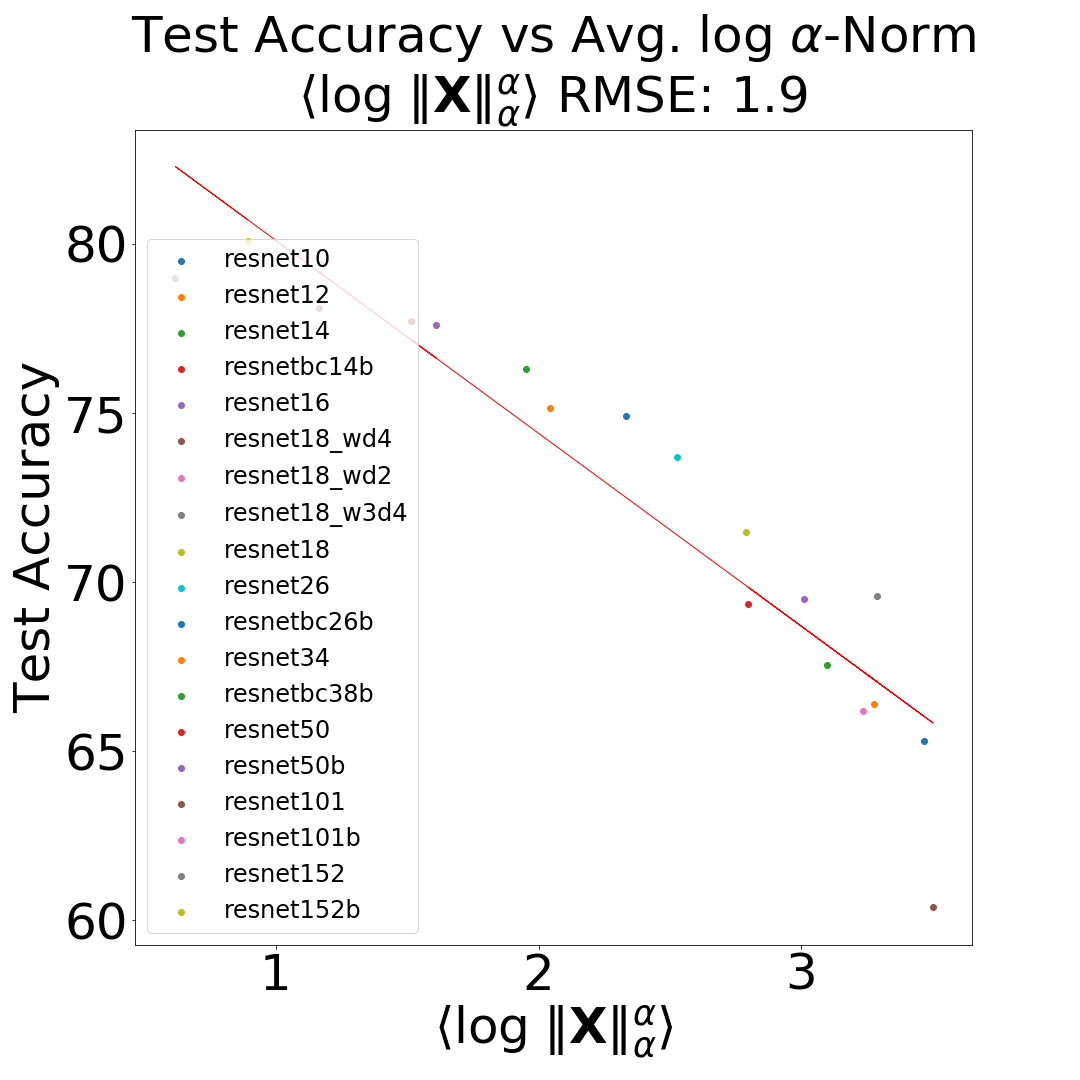
\includegraphics[width=4.5cm]{img/ResNet-1K_logpnorm_accs.png}
        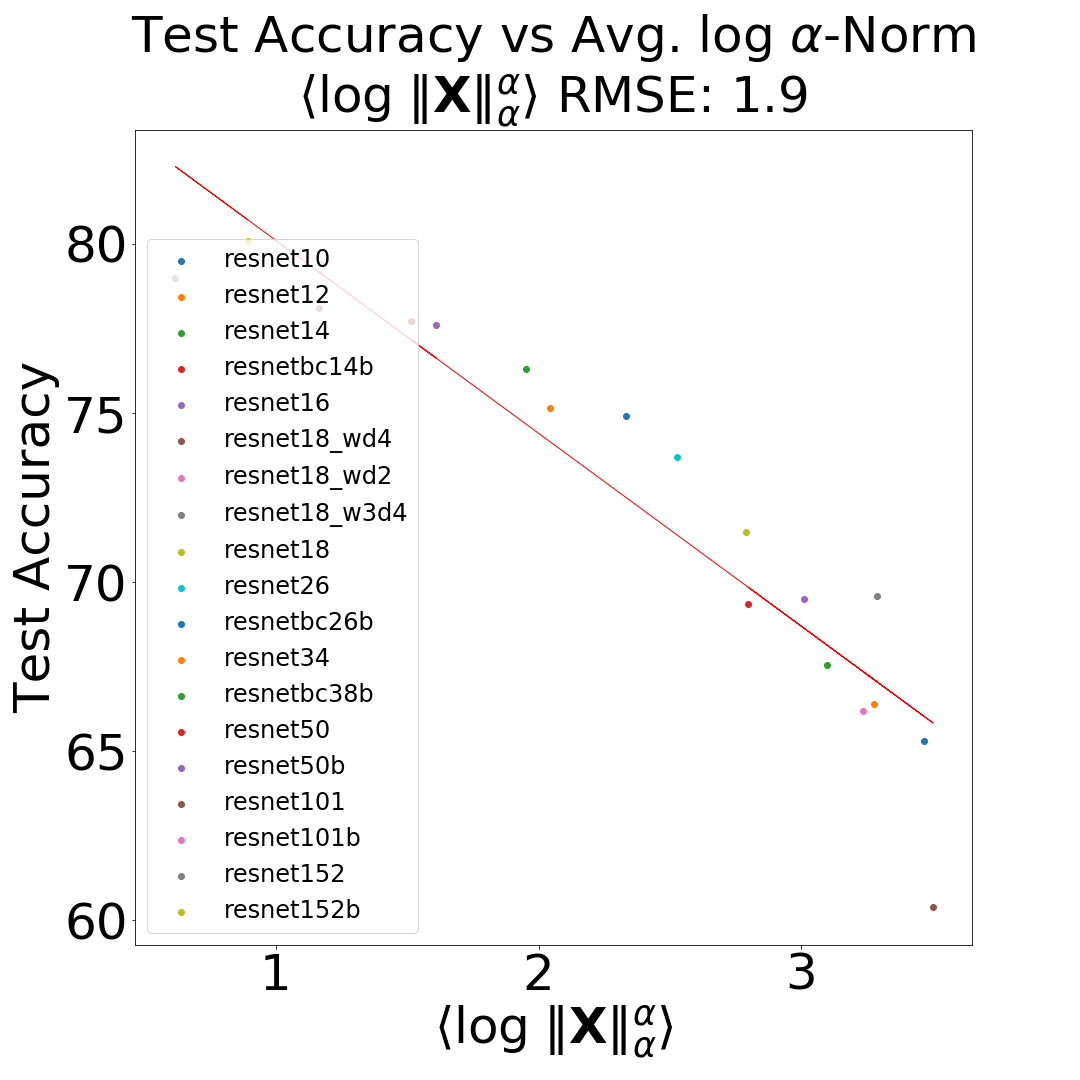
\includegraphics[width=3.7cm]{img/ResNet-1K_logpnorm_accs.png}
        \label{fig:resnet1k-accuracy}
    }
    \qquad
    \subfigure[ DenseNet, $\alpha$-Norm ]{
        %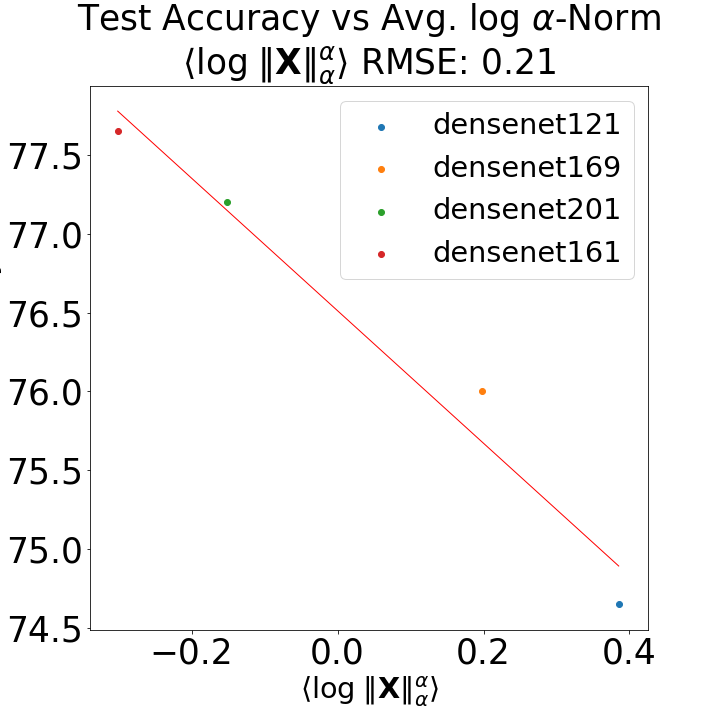
\includegraphics[width=4.4cm]{img/DenseNet_logpnorm_accs.png}
        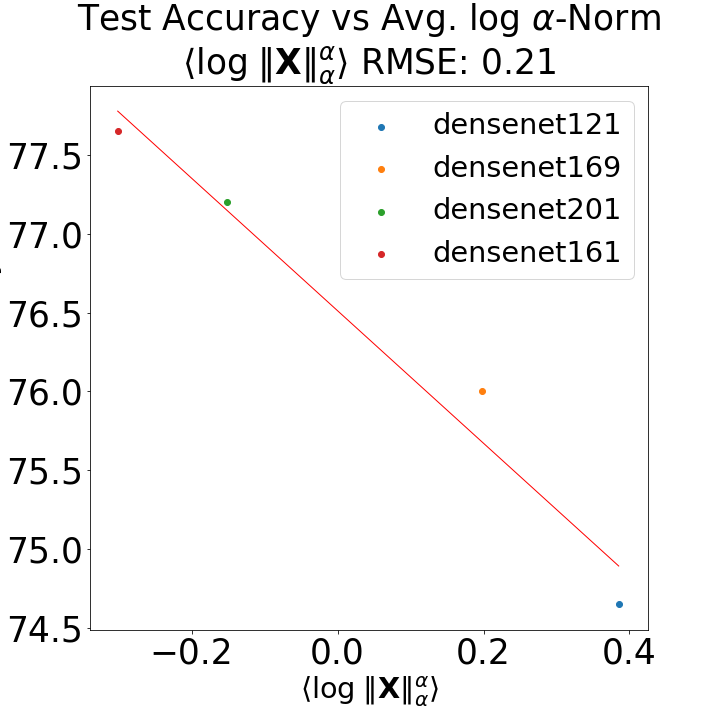
\includegraphics[width=3.7cm]{img/DenseNet_logpnorm_accs.png}
        \label{fig:densenet-accuracy}
    }
    \caption{$\alpha$-Norm versus reported Top1 Error for  ResNet, ResNet-1K, and DenseNet models. The corresponding results for VGG are shown in Figure~\ref{fig:vgg-pnorm}.  }
    \label{fig:cv2-accuracy}
\end{figure}


\begin{table}[t]
\small
\begin{center}
%\begin{tabular}{|p{1in}|c|c|c|c|c|}
\begin{tabular}{|p{0.75in}|c|c|c|c|c|}
%\begin{tabular}{|l|c|c|c|c|c|}
\hline
%   &    & Frobenius Norm & Spectral Norm & Weighted Alpha & Alpha-Norm \\
% Series & \#Models   & $\Vert\mathbf{W}\Vert_{F}$ & $\Vert\mathbf{W}\Vert_{\infty}$ & $\hat{\alpha}=\alpha\log\lambda_{max}$ & $\Vert\mathbf{X}\Vert^{\alpha}_{\alpha}$ \\
        & Num.   & $\Vert\mathbf{W}\Vert_{F}$ & $\Vert\mathbf{W}\Vert_{\infty}$ & $\hat{\alpha}$ & $\Vert\mathbf{X}\Vert^{\alpha}_{\alpha}$ \\
 Series & Models & Metric                     & Metric                     & Metric         & Metric                                   \\
\hline
 VGG       &  6 & 0.56 & 0.53 & 0.48          & \textbf{0.42}  \\
 ResNet    &  5 & 0.9  & 1.4  & \textbf{0.61} & 0.66           \\
 ResNet-1K & 19 & 2.4  & 3.6  & \textbf{1.8}  & 1.9            \\
 DenseNet  &  4 & 0.3  & 0.26 & \textbf{0.16} & 0.21           \\
\hline
\end{tabular}
\end{center}
\caption{RMSE (smaller is better) for linear fits of quality metrics to Reported Top1 Test Error for pretrained models in each architecture series.  VGG, ResNet, and DenseNet were pretrained on ImageNet, and ResNet-1K was pretrained on ImageNet-1K. 
\michael{Are the numbers in this table stale; if they get updated, then we need to modify the test at at least two places, on actual numbers and on what is best.}
}
\label{table:cv-models}
\end{table}


Figure~\ref{fig:cv2-accuracy} plots the 
%overall best performing (i.e., 
Log $\alpha$-Norm
%) 
metric for the full ResNet, ResNet-1K, and DenseNet series.
(A much more detailed set of plots, including the behavior of all four methods on each of the series, is available at \cite{XXX-WEB-LINK}.)
Here, the Log $\alpha$-Norm is much better that the Log Frobenius/Spectral norm metrics (although, as Table~\ref{table:cv-models} shows, it is actually slightly worse than the Weighted Alpha metric).
Notice also that ResNet series, which has been trained on the full ImageNet dataset, has an RMSE of $0.66$, whereas the ResNet-1K series, which has been trained on the much smaller ImageNet-1K dataset, also correlated wells, but has a much larger RMSE of $1.9$.

See Table~\ref{table:cv-models} for a summary of results for Top1 Accuracies for all four metrics on all four model series.
Similar results (not shown) are obtained for the Top5 Accuracies.
Overall, for the the ResNet, ResNet-1K, and DenseNet series, all metrics perform relatively well, the Log $\alpha$-Norm metric performs second best, and the Weighted Alpha metric performs best. 
These model series are all well-trodden, and our results indicate that norm-based metrics and PL-based metrics can both distinguish among ``good-better-best'' models, with PL-based metrics performing somewhat better. 


\paragraph{Layer Analysis: Correlation Flow in CV Models.}

We can learn much more about a pretrained model by going beyond average values to examining quality metrics for each layer weight matrix, $\mathbf{W}$, as a function of depth (or layer id).  % in the network. 
%The most interesting results are seen when we 
For example, we can 
plot \nred{just} the PL exponent, $\alpha$,%
\footnote{That is, here we consider just $\alpha$ for each layer, not $\hat{\alpha}$ or $\Vert\mathbf{W}\Vert^{\alpha}_{\alpha}$.} 
as a function of depth.
%
See Figure~\ref{fig:vgg-alpha-layers}, which plots $\alpha$ for each layer (the first layer corresponds to data, the last layer to labels) for the least accurate (shallowest) and most accurate (deepest) model in each of the VGG (without BatchNormalization), ResNet-1K, and DenseNet series.
(Again, much more detailed set of plots is available at \cite{XXX-WEB-LINK}; but note that the corresponding layer-wise plots for Frobenius and Spectral norms are much less interesting than the results we present here.)

\begin{figure}[t]
    \centering

    \subfigure[ VGG ]{
        %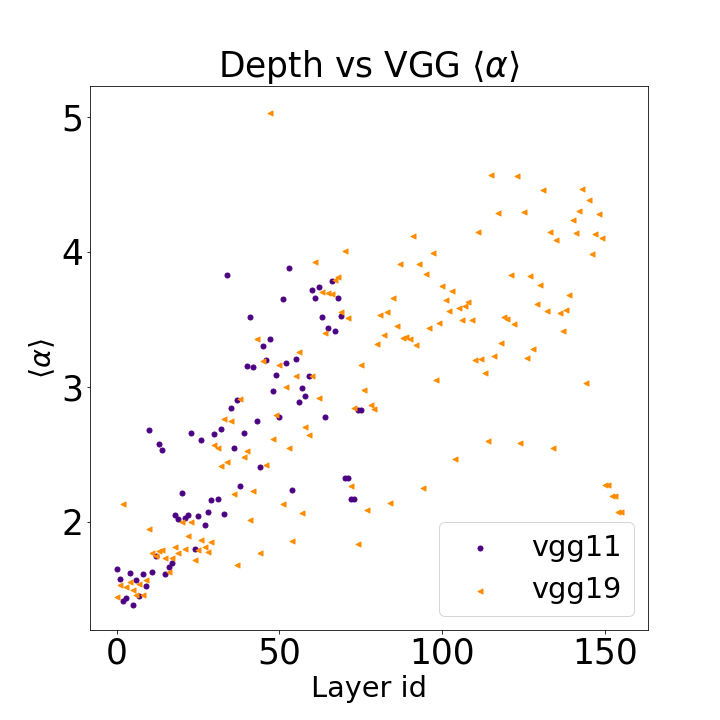
\includegraphics[width=4.5cm]{img/VGG_fnl_alpha_depth.png} 
        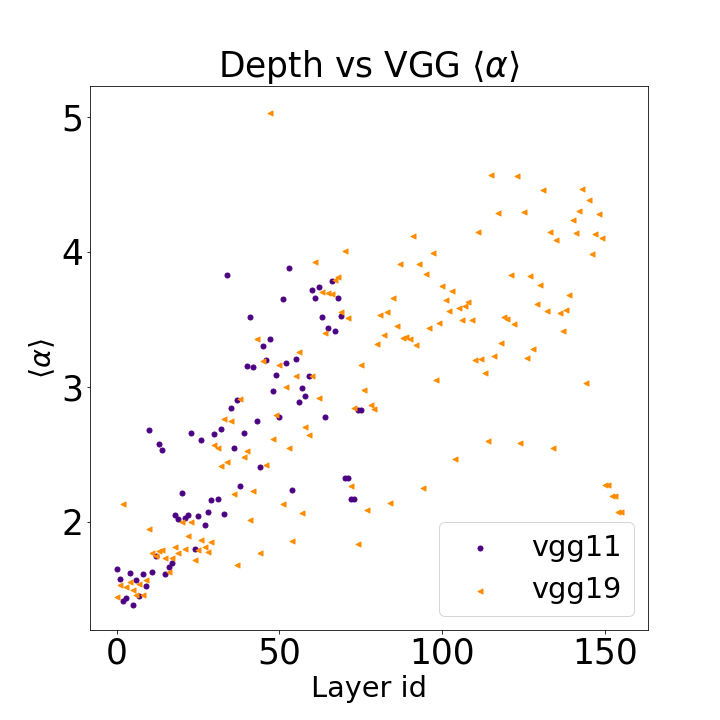
\includegraphics[width=3.7cm]{img/VGG_fnl_alpha_depth.png} 
                \label{fig:vgg-alpha-layers}
    }
    \qquad
    \subfigure[ ResNet-1K ]{
        %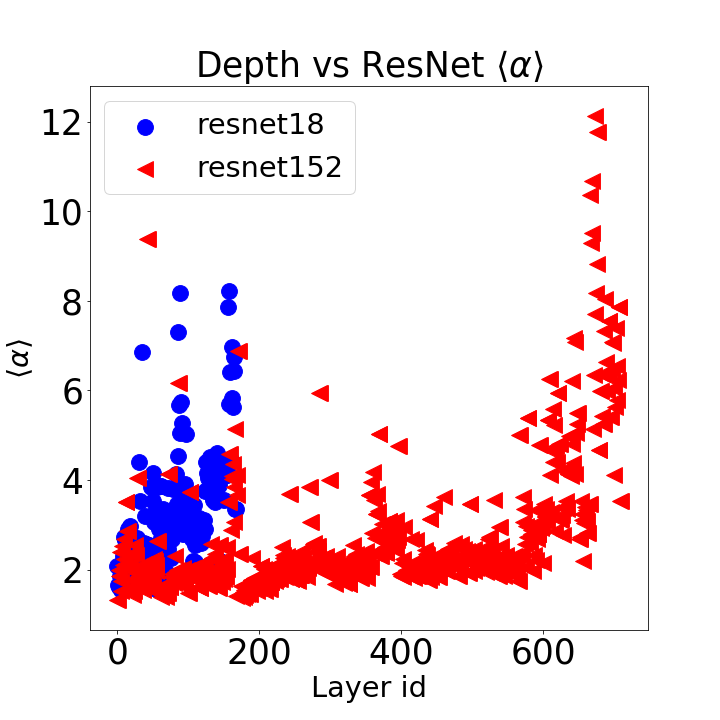
\includegraphics[width=4.5cm]{img/ResNet_fnl_alpha_depth.png} 
        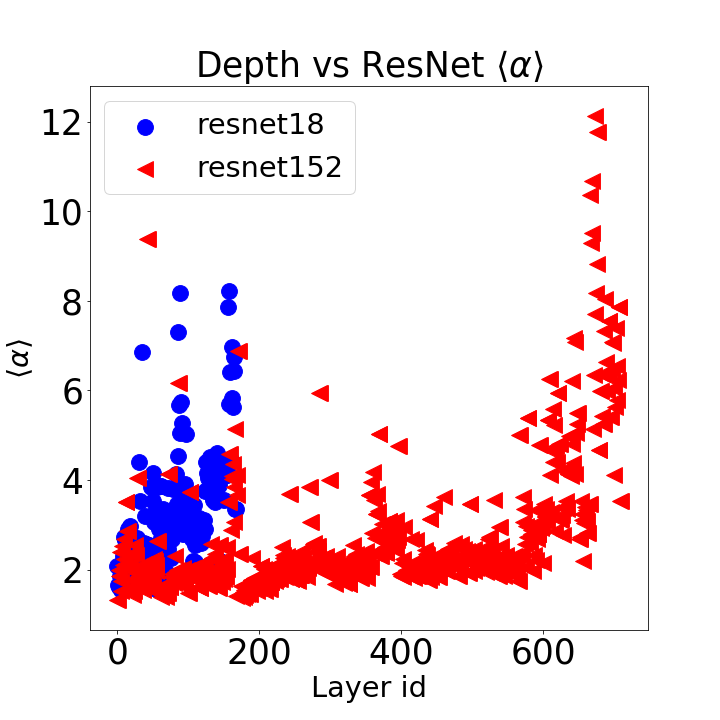
\includegraphics[width=3.7cm]{img/ResNet_fnl_alpha_depth.png} 
        \label{fig:resnet-alpha-layer}
    }
    \qquad
    \subfigure[ DenseNet ]{
        %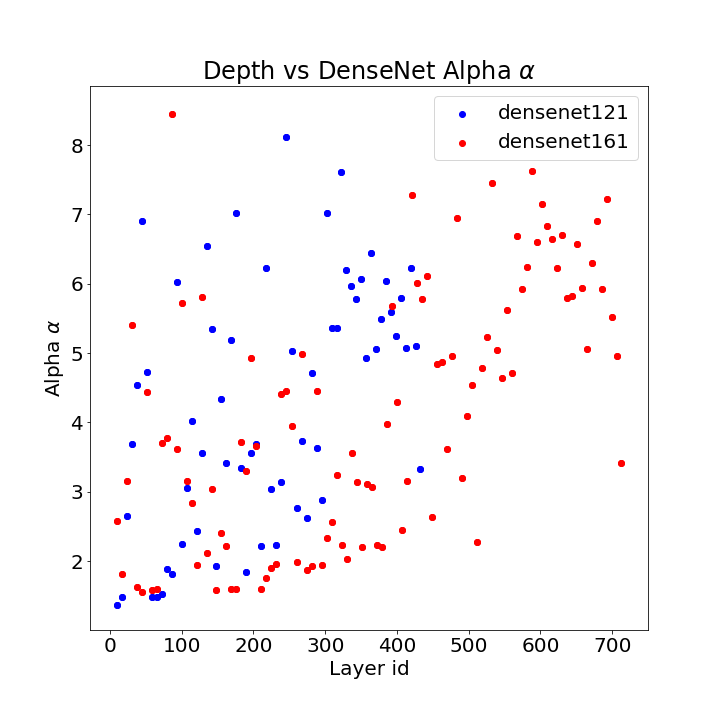
\includegraphics[width=4.5cm]{img/DenseNet_fnl_alpha_depth.png} 
        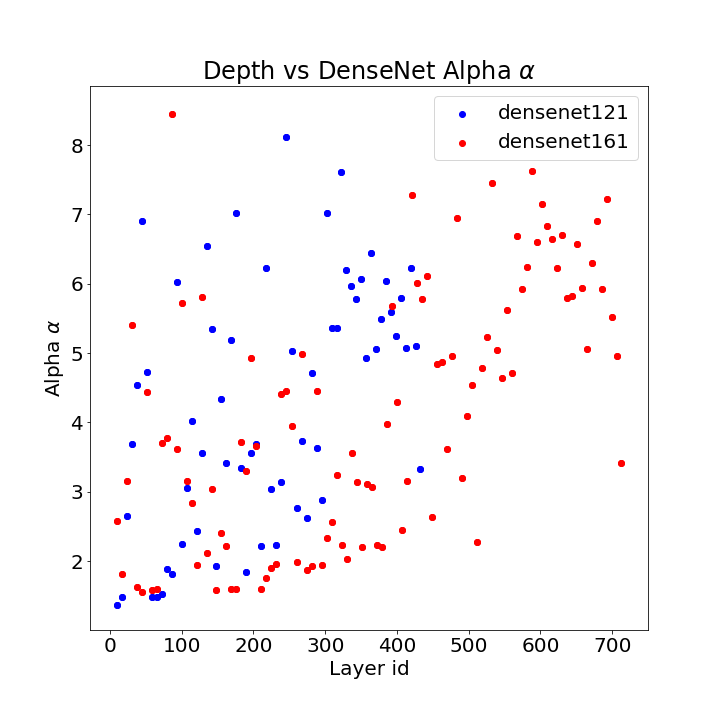
\includegraphics[width=3.7cm]{img/DenseNet_fnl_alpha_depth.png} 
        \label{fig:densenet-alpha-layer}
    }
    \caption{Layer Analysis. 
             PL exponent $\alpha$ versus layer id, for VGG, ResNet-1K, and DenseNet models.  
             (Y axes on each plot are different.)  
             ResNet-1K exhibits different and much more stable behavior across layers.
             This contrasts with how VGG gets gradually worse in deeper layers and how DenseNet is worse and much more erratic.  
             We interpret this in the text as quantifying a \emph{correlation flow} across the layers.  
            }
    \label{fig:vgg-alpha-layers}
\end{figure}

In the VGG models, Figure~\ref{fig:vgg-alpha-layers} shows that the PL exponent $\alpha$ systematically increases as we move down the network, from data to labels, in the Conv2D layers, starting with $\alpha\lesssim 2.0$ and reaching all the way to $\alpha\sim 5.0$; and then, in the last three, large, fully-connected (FC) layers, $\alpha$ stabilizes back down to $\alpha\in[2,2.5]$.
This is seen for all the VGG models (again, only the shallowest and deepest are shown in this figure), indicating that the main effect of increasing depth is to increase the range over which $\alpha$ increases, thus leading to larger $\alpha$ values in later Conv2D layers of the VGG models.
This is quite different than the behavior of either the ResNet-1K models or the DenseNet models.

For the ResNet-1K models, $\alpha$ also increases in the last few layers (more dramatically, in fact, observe the differing scales on the Y axes).
However, as the ResNet-1K models get deeper, there is a wide range over which $\alpha$ values tend to remain small.
\michael{Can we say something about exceptions which are larger than for VGG or DenseNet.}
\charles{You have the same plots I do..what do you want to say >}
\michael{Are they small or different types of layers or something?}
\charles{Not that I am aware of.  Ill think on it}
This is seen for other models in the ResNet-1K series, but it is most pronounced for the larger ResNet-1K (152) model, where $\alpha$ remains relatively stable at $\alpha\sim 2.0$, from the earliest layers all the way until we reach close to the final layers.  

For the DenseNet models, $\alpha$ tends to increase as the layer id increases, in particular for layers toward the end.
While this is similar to what is seen in the VGG models, with the DenseNet models, $\alpha$ values increase almost immediately after the first few layers, and the variance is much larger (in particular for the earlier and middle layers, where it can range all the way to $\alpha\lesssim 8.0$) and much less systematic throughout the network.

Recall the differences---in particular, the number of residual connections---between the VGG, ResNet, and DenseNet architectures.
VGG, while a fine model in many ways, was limited by needing massive FC layers at the end of the model, requiring significant memory and computational resources, and it's poor conditioning led to problems with vanishing gradients.  
The empirical manifestations of this (on weight matrices) are that fitted $\alpha$ values get much worse for deeper layers.
ResNet greatly improved on VGG by introducing residual connections, allowing for greater accurary with far fewer parameters.
(Indeed, ResNet models of up to 1000 layers have been trained.) 
We conjuecture that the effeciency and effectivness of ResNet is reflected in the smaller and more stable $\alpha\sim 2.0$, across nearly all layers, indicating that the inner layers are very well correlated and strongly optimized.
This should also be contrasted with the DenseNet model, which contains many connections between every layer.
Our results (large $\alpha$, meaning they even a HT model is probably a poor fit) suggest that DenseNet has too many connections, diluting high quality interactions across layers, and leaving many layers very poorly optimized.

More generally, we can understand Figure~\ref{fig:vgg-alpha-layers} in terms of the \emph{flow of correlation}, as follows.
Recall that the Log $\alpha$-Norm metric and the Weighted Alpha metric are based on HT-SR Theory~\cite{MM18_TR, MM19_HTSR_ICML, MM20_SDM}, which is in turn based on ideas from the statisical mechanics of heavy tailed and strongly correlated systems~\cite{BouchaudPotters03, SornetteBook, BP11, bun2017}. 
There, one expects well-trained systems which exhibit correlations over many size scales to have ESDs that can be well-fit by PLs, with PL exponents $\alpha\approx 2$.
Much larger values of $\alpha$ indicate very poor fits, but the presence of many adjacent layers with relatively good PL fits \emph{suggests} that those adjacent layers ``impedance match'' well and that the correlations that are captured by one layer propagate well to subsequent layers.
Informally, one would expect a DNN model to perform well when it fascilitates the propagation of information/features across layers.
In the absence of training/test data, we can to try to quantify this by measuring the PL properties of empirical weight matrices.
Smaller $\alpha$ values correspond to layers in which correlations across multiple scales are better captured~\cite{MM18_TR,SornetteBook}, and thus we expect that small values of $\alpha$ that are stable across multiple layers enable better \emph{correlation flow} through the network.


%\paragraph{Layer Analysis: Behavior on Less Thoroughy Studied CV Models.}
\paragraph{Layer Analysis: Differences Between PL Metrics and Norm Metrics.}

The similarity between norm-based metrics and $\alpha$-based metrics suggests a question: is the Weighted Alpha metric just a variation of the more familiar norm-based metrics, or does it capture something different?  
More generally, do fitted $\alpha$ values contain information not captured by norms? 
To show that it is not just a variation and that $\alpha$ does capture something different, consider the following example, which looks at a compressed / distilled DNN model~\cite{CWZZ17_TR}.


\begin{figure}[t]
   \centering
   \subfigure[$\lambda_{max}$ for ResNet20 layers]{
      %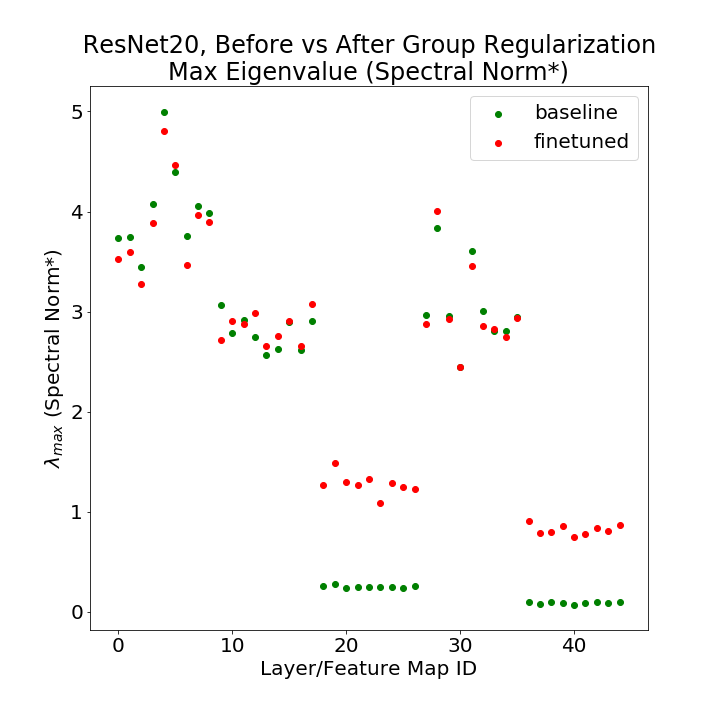
\includegraphics[scale=0.14]{img/resnet4d_maxev.png}
      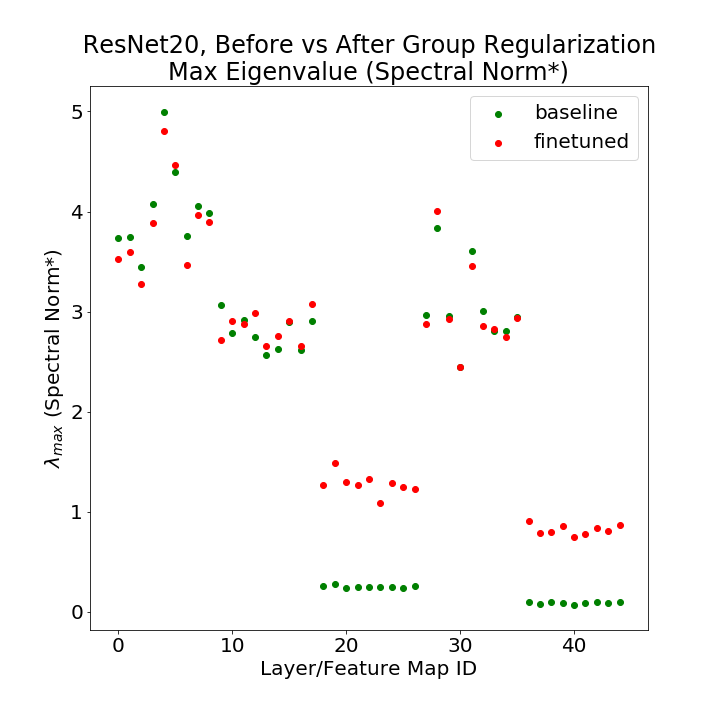
\includegraphics[width=3.7cm]{img/resnet4d_maxev.png}
      %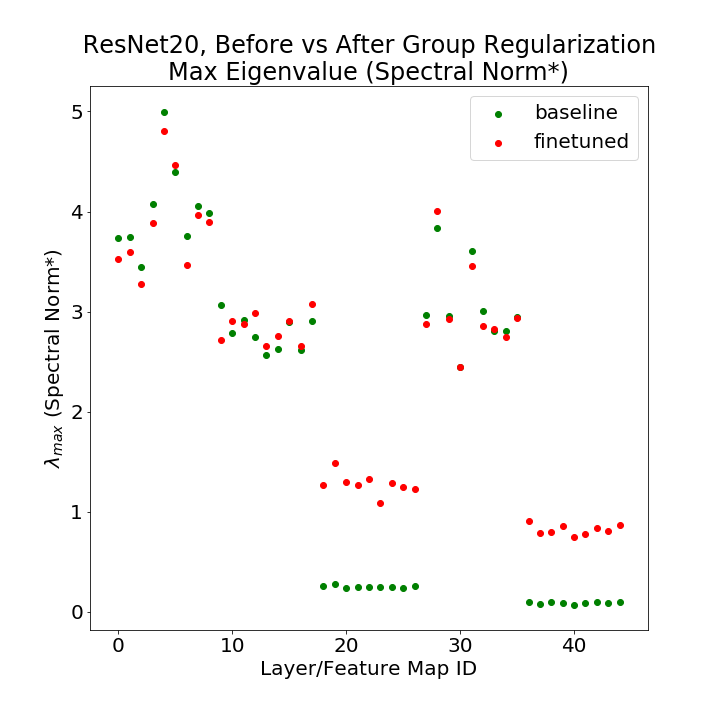
\includegraphics[width=4.5cm]{img/resnet4d_maxev.png}
      \label{fig:resnet204Dalpha}
   }
   \qquad
   \subfigure[$\alpha$ for ResNet20 layers]{
      %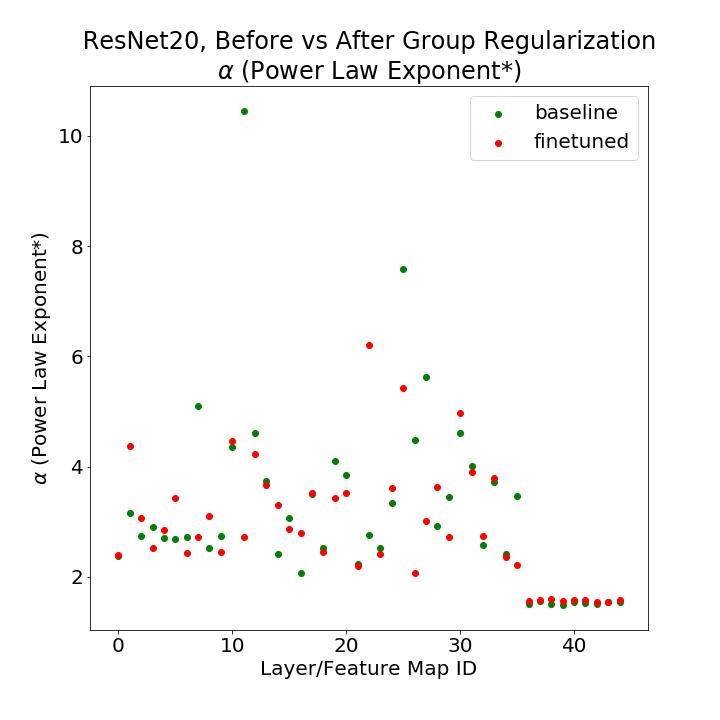
\includegraphics[scale=0.14]{img/resnet4d_alphas.png}
      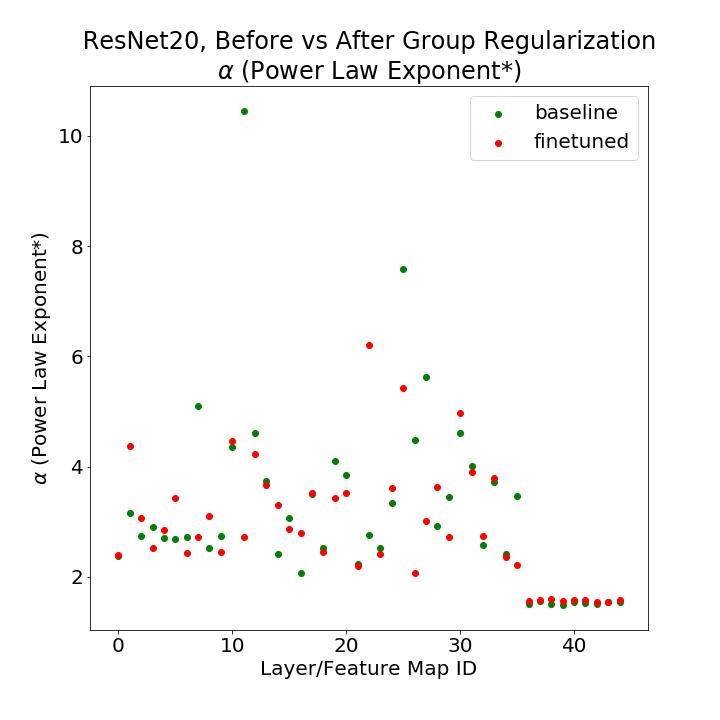
\includegraphics[width=3.7cm]{img/resnet4d_alphas.png}
      %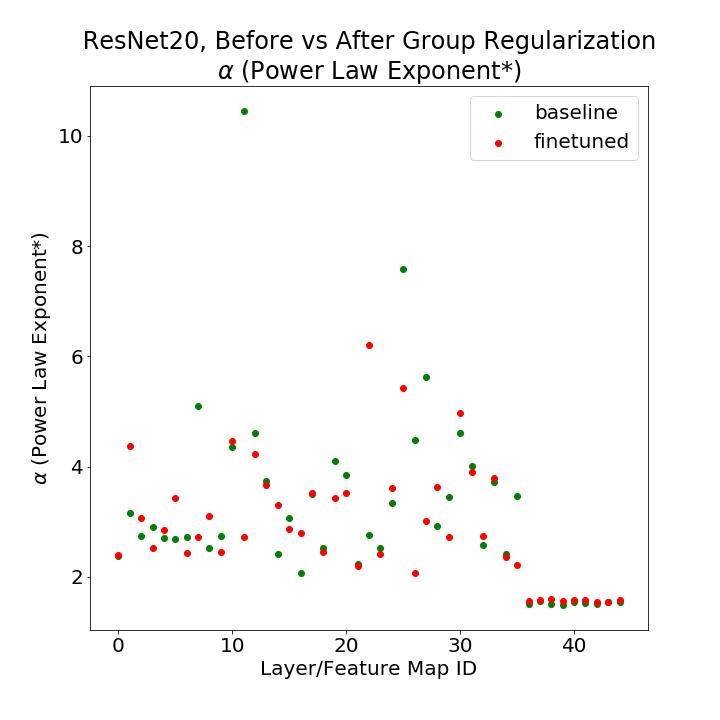
\includegraphics[width=4.5cm]{img/resnet4d_alphas.png}
      \label{fig:resnet204Dmaxev}
   }
   \caption{Layer Analysis.
            ResNet20, distilled with Group Regularization, as implemented in the \texttt{distiller} (4D\_regularized\_5Lremoved) pre-trained models.  
            Spectral Norm, $\lambda_{max}$, and, PL exponent, $\alpha$, for individual layer, versus layer id, for both between baseline (before distillation, shown in green) and fine-tuned (after distillation, shown in red) pre-trained models. 
           }
   \label{fig:resnet204D5L}
\end{figure}

We consider ResNet20, trained on CIFAR10, before and after applying the Group Regularization technique, as implemented in the \texttt{distiller} package.%
\footnote{For details, see \url{https://nervanasystems.github.io/distiller/\#distiller-documentation} and also \url{https://github.com/NervanaSystems/distiller}.}
We analyze the available pre-trained 4D\_regularized\_5Lremoved baseline and fine-tuned models.  %\cite{distiller_repo}.
The reported baseline test accuracies ($Top1=91.45$ and $Top5=99.75$) are better than the reported fine-tuned test accuracies ($Top1=91.02$ and $Top5=99.67$)~\cite{XXX-XXX}.
The previous results on ResNet (Table~\ref{table:cv-models} and Figure~\ref{fig:cv2-accuracy} might suggest that the baseline Spectral Norm should be \emph{smaller} than those of the layers in the fine-tuned model.
\michael{Do we have something backwards here: where we observed that the average norm to increase with decreasing test error (as it ``should'' not), whereas the average PL exponent $\alpha$ decreases (as ``expected'' from HT-SR Theory).  }
In both cases (Frobenius norm results not shown), we observe the opposite.
Figure~\ref{fig:resnet204D5L} presents the Spectral Norm ($\lambda_{max}$) and PL exponent ($\alpha$) for each individual layer weight matrix $\mathbf{W}_{l}$.%
\footnote{Here, we only include layer matrices or feature maps with $M\ge50$.}
On the other hand, the $\alpha$ values do not differ systematically between the baseline and fine-tuned models.
\michael{Some comment about big jump in norm; but fix previous backwards question first.}
Also (not shown), the average (unweighted) baseline $\alpha$ is \emph{smaller} than the fine-tuned average (as would be predicted by HT-SR Theory, on which $\hat{\alpha}$ is based).


\michael{XXX.  WORK ON THIS PAR AFTER DO NLP EXAMPLES.}
Our interpretation of this is the following.
The pre-trained models in the \texttt{distiller} package have passed some quality metric, but they are much less well trodden than any of the VGG/ResNet/DenseNet models we condisered previously.
Norms are often used as regularizers, and thys they are a natural metric to consider, e.g., during training or distillation.
The PL $\alpha$ captures more subtle correlations.
%
The reason for this is that the \texttt{distiller} Group Regularization technique has the unusual effect of increasing the norms of the $\mathbf{W}$ feature maps for at least two of the Conv2D layers.
\michael{This impedance shuffling or whatever it is called messes up norms, but the strong correlations are still preserved, as seen in the $\hat{\alpha}$ metric, and the model quality is good.  CLARIFY.}
\michael{XXX.  INTERPRET IN TERMS OF XXX GOOD VERSUS BAD, AS OPPOSED TO GOOD BETTER BEST.}


